\documentclass[../eatbrain.tex]{subfile}

\subsection{Struttura}
\label{sec-struttura}
Grazie alla tipologia di contenuto presente nel sito la struttura generale di quest'ultimo risulta semplice e abbastanza lineare:  ogni sezione infatti presenta al massimo due livelli di profondità, rendendo disponibile l'informazione ricercata in al massimo due click (avendo un'idea precisa di ciò che si vuole trovare). \\
Questa caratteristica è molto utile: l'utente spesso dopo 3 click tende a interrompere la ricerca, provando frustrazione e diminuendo la probabilità di tornare a vistiare il sito.\\
La struttura delle singole pagine è invece uguale per tutte: esclusa la home page che fa una panoramica di tutte le sezioni e necessita di un two columns layout\footnote{http://www.webstyleguide.com/wsg3/6-page-structure/4-page-templates.html} (lasciando il contenuto più corposo nella colonna di sinistra, migliorandone la visibilità), le pagine interne sono disposte ad una colonna sola, rendendo di facile individuazione il contenuto cercato. \\
Le pagine interne di primo livello (quelle collegate direttamente al menù), dovendo esporre un elenco di dati, presentano uno schema a griglia (immagine + titolo) che risulta più efficace di una semplice lista. \\
Un altro punto a favore lo si trova nel layout generico: tutte le pagine infatti hanno uno schema fisso: \\\\
\begin{figure}[h]
	\centering
	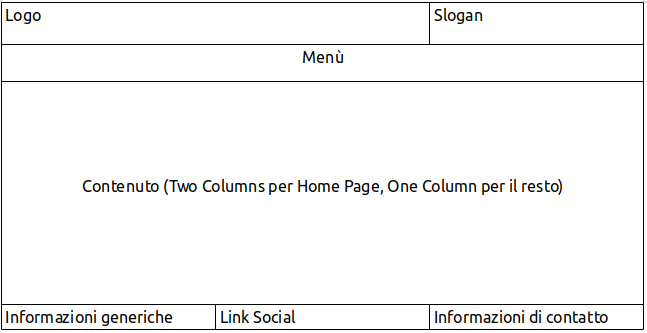
\includegraphics[width=12cm,height=6cm]{immagini/struttura}
	\caption{Struttura generica di tutte le pagine}
	\label{struttura-default}
\end{figure}\\\\
Facilitando l'orientamento all'interno del sito dopo poche interazioni.
\newpage
\subsection{Navigazione}
\label{sec-nav}
La navigazione interna risulta molto semplice ed efficace, nonostante l'assenza di un breadcrumb per specificare con esattezza la propria posizione all'interno del sito, la struttura poco profonda del sito permette di non sentirne la mancanza. Inoltre il menù evidenzia la sezione in cui ci si trova permettendo all'utente di rendersi conto immediatamente della propria posizione.\\
Volendo essere pignoli, lo strumento utilizzato per evidenziare la sezione (i triangolini rivolti verso l'alto) può confondersi nella home page (in quanto molto vicino al logo che è simile) ma una volta cambiata sezione l'associazione è immediata. In più ogni pagina interna presenta come prima riga del contenuto il titolo della sezione permettendo di essere sempre consci della pagina che si sta visitando.
\begin{figure}[h]
	\centering
	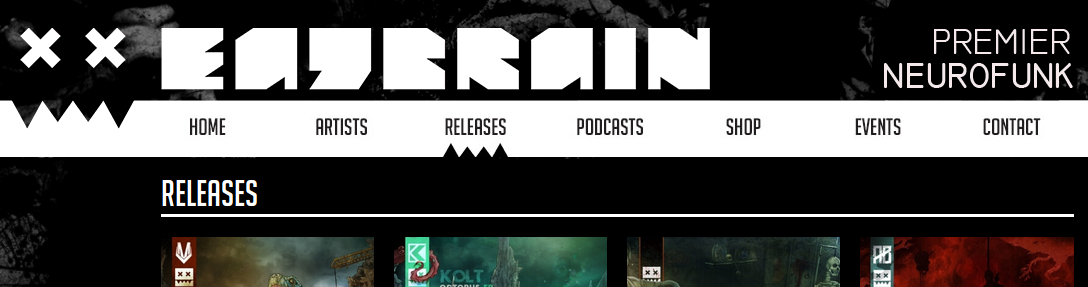
\includegraphics[width=12cm]{immagini/menu}
	\label{menu}
	\caption{Menu nella pagina "Releases"}
\end{figure}\\
Un'altra piccolezza molto importante è che per navigare tra le pagine non viene richiesto nessun dato o aperta nessuna nuova finestra, rendendo possibile il viaggio nel tempo all'indietro senza alcuna limitazione. Questa caratteristica è molto importante perchè gli utenti preferiscono cliccare fino a 7 volte il tasto back del browser piuttosto che cercare un link diretto, questo sito quindi lascia l'opportunità di cliccare back per tutte le volte necessarie a ritrovare l'informazione.\\
Il menù inoltre è molto accessibile: grazie alla struttura semplice della pagina non sono presenti menù a cascata che possono risultare fastidiosi con troppi livelli di profondità, mentre i tasti disponibili sono ben visibili e facilmente cliccabili (lo spazio per il click è sufficiente).
Alcuni problemi possono trovarsi nell'individuazione dei link, ma il discorsò verrà approfondito nella sezione \hyperref[convenzioni]{\texttt{Rispetto Delle Convenzioni}}.
\subsection{Ricerca}
Nel sito è completamente assente la funzionalità di ricerca, sebbene questo può non essere un problema nelle pagine principali, può causare sensazioni negative nelle pagine a profondità più bassa: come dicevamo prima le pagine che elencano artisti e tracce musicali sono disposte a griglia e non hanno un numero limitato di elementi; questo può causare frustrazione nell'utente quando impegnato nella ricerca di un determinato artista: la disposizione della pagina lo obbliga ad effettuare lo scroll verticale e a sforzare la testa per individuare l'elemento ricercato.\\
Inoltre le tracce audio sono disposte in ordine cronologico (a differenza degli artisti che seguono l'ordine alfabetico) senza esplicitare l'effettiva data d'uscita, richiedendo all'utente lo sforzo aggiuntivo di ricordare a grandi linee il periodo di pubblicazione della traccia desiderata. \\
Un elemento che può ridurre questo problema è lo strumento di ricerca del browser ma anche questo richiede sforzo per la sua attivazione e l'utente può non esserne a conoscenza.
\subsection{Contenuti Multimediali}
\label{multimedia}
Essendo un portale volto alla promozione di contenuti musicali, la scelta di proporre contenuto multimediale pare essere quella più ovvia, questa integrazione è stata fatta in modo molto buono dagli sviluppatori ma non è esente da pecche.\\
\subsubsection{Lati Negativi}
Lo slideshow, ad esempio, risulta essere un gran tallone d'achille per il sito: questo occupa gran parte della home page ma non offre alcuna informazione significativa, anzi può causare disorientamento nell'utente. Le immagini proposte sono infatti una panoramica delle ultime news ma, nonostante lo scorrimento abbia tempi buoni e viene offerto un sistema di controllo per l'utente (freccette direzionali), non sono accompagnate da nessun testo e cosa ancora più grave non sono cliccabili, infondendo solo confusione nell'utente. In più lo slideshow occupa 3/4 della parte visibile della home page occupando i timer dell'utente in modo fin troppo invasivo (come vedremo nel dettaglio dell'analisi della \hyperref[sec-home-page]{\texttt{Home Page}}).
Altro problema più lieve è quello di usare un'immagine come segnalatore di pagina (i triangolini di cui parlavamo sopra): in presenza di connessioni ad internet molto lente questo può non mostrarsi nell'immediato disorientando l'utente, un problema comunque molto lieve.
Ultimo problema (ancora più lieve) è lo slogan, essenzialmente sono due parole ma la sua rappresentazione tramite immagine preclude la possibilità di \texttt{copy\&paste} per gli utenti più pigri, che potrebbero frustrarsi.\\
\begin{figure}[h]
	\centering
	
\includegraphics[width=6cm]{immagini/slogan}
	\caption{Slogan della compagnia}
	\label{slogan-img}
\end{figure}
\newpage
\subsubsection{Lati Positivi}
Passando ai lati positivi (questo in particolare estremamente positivo) merita una menzione l'integrazione con il servizio di streaming audio \texttt{Soundcloud}: in ogni pagina di artista o release il sito offre la possibilità di ascoltare la musica tramite \texttt{Soundcloud} senza abbandonare il portale, suscitando gratificazione immediata all'utente che potrà usufruire del contenuto desiderato senza abbandonare la pagina che sta visitando. Inoltre la scelta di ascoltare la musica è affidata completamente all'utente: non parte in automatico. \\
Se proprio dobbiamo trovarci una pecca è che browser senza javascript non solo non potranno usufruire del servizio di \texttt{Soundcloud} ma non verranno nemmeno avvisati della possibilità di farlo, osservando semplicemente uno spazio nero.
\begin{figure}[h]
	\centering
	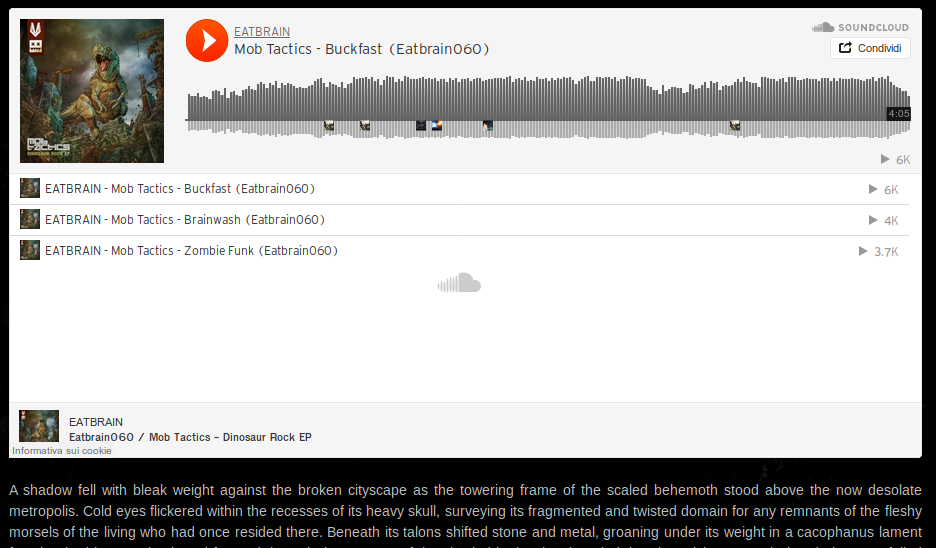
\includegraphics[width=12cm]{immagini/soundcloud}
	\caption{Integrazione con Soundcloud}
	\label{soundcloud-integration}
\end{figure}\\
Altro lato positivo è l'immagine di sfondo, questa infatti si integra perfettamente con il design del sito e non appesantisce la fruizione dello stesso. \\
Come vedremo più avanti il portale rompe la convenzione del visited link, rendendo più difficile l'individuazione dei contenuti già visitati, fortunatamente le immagini vengono in nostro aiuto: le release di tracce, sia nella home page che nella sezione dedicata, sono accompagnate dall'immagine di copertina, questo può aiutare nell'individuazione di eventuali novità: è più facile ricordarsi un immagine che un testo (titolo della release).
\subsection{Rispetto Delle Convenzioni}
\label{convenzioni}
\subsubsection{Convenzioni Esterne}
Nonostante il sito cerchi di avvicinarsi al mondo che la musica neurofunk rappresenta, non si presenta il fenomeno di bloated design:
la navigazione infatti rimane scorrevole e le scelte stilistiche particolari si adattano bene alla struttura del sito, inoltre, essendo il portale atto a promuovere musica, non cade nell'errore dell'avvio automatico di tracce musicali: come, quando e perché ascoltare musica è completamente deciso dall'utente. \\
Un problema invece lo troviamo nei link: il colore del testo normale e dei link non discosta di molto e link visitati non sono diversi da quelli non ancora cliccati. \\
Dove invece si aumenta il contrasto tra collegamenti e testo normale (blocchi di testo molto grandi, eg: descrizioni artisti/release) l'utente cade in una nuova trappola: il colore dei link è uguale al colore delle parole chiave del testo, causando confusione e frustrazione al mancato evento successivo al click di un presunto link (rottura della metafora visiva).\\
\begin{figure}[h]
	\centering
	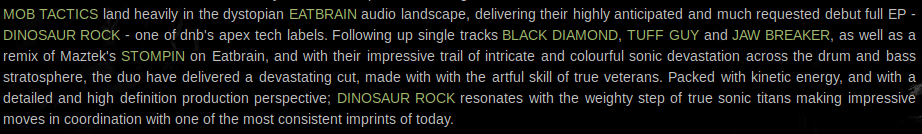
\includegraphics[width=12cm]{immagini/non-link}
	\caption{Esempio di link  cliccabili e non cliccabili}
	\label{non-link}
\end{figure}\\
Come vediamo nell'immagine sopra ad esempio, solo i primi tre link di colore verdi sono cliccabili, le restanti sono semplici parole chiave del testo. Inoltre le parole \texttt{Dinosaur Rock} sono cliccabili nel primo caso e non cliccabili nel secondo, causando ancora più confusione e frustrazione.
\subsubsection{Convezioni Interne}
Sebbene le convenzioni esterne siano discretamente rispettate, c'è una mancanza leggermente più grave nelle convenzioni interne del sito: in casi di contenuto informativo simile i link a volte sono posti sui titoletti mentre altre sulle immagini. Questa discrepanza può rompere la mappa mentale che l'utente si è fatto del sito, diminuendo la certezza che al click si scateni un evento. \\
Un esempio possiamo trovarlo nelle pagine \texttt{Artists} e \texttt{Releases}: entrambe presentano una lista a griglia ma nella prima per accedere al contenuto in dettaglio è sufficiente cliccare sull'immagine, nella seconda invece bisogna cliccare sul testo immediatamente sotto (ignorando inoltre la legge di Fitt\footnote{https://it.wikipedia.org/wiki/Legge\_di\_Fitts}).
\subsection{Gestione degli Errori}
Capita a tutti gli utenti di cliccare su un link che indirizza ad una pagina non esistente, che sia un link sbagliato o un contenuto rimosso la situazione può essere frustrante per un utente meno esperto, soprattutto quando il link incriminato è all'interno del sito. \\
Fortunatamente sul sito di Eatbrain non ci sono link "corrotti" ma è possibile che siti esterni indirizzino a pagine del sito che non esistono più. Per ovviare a questo problema gli sviluppatori di \texttt{eatbrain.net} hanno sviluppato una pagina di 404 (l'errore standard dell'http per il contenuto non trovato) personalizzata, che mantiene lo stesso layout del sito evitando di lasciare nell'utente la sensazione di smarrimento, offrendo il menu di navigazione per permettere all'utente di navigare nelle altre sezioni del sito.\\
\begin{figure}[h]
	\centering
	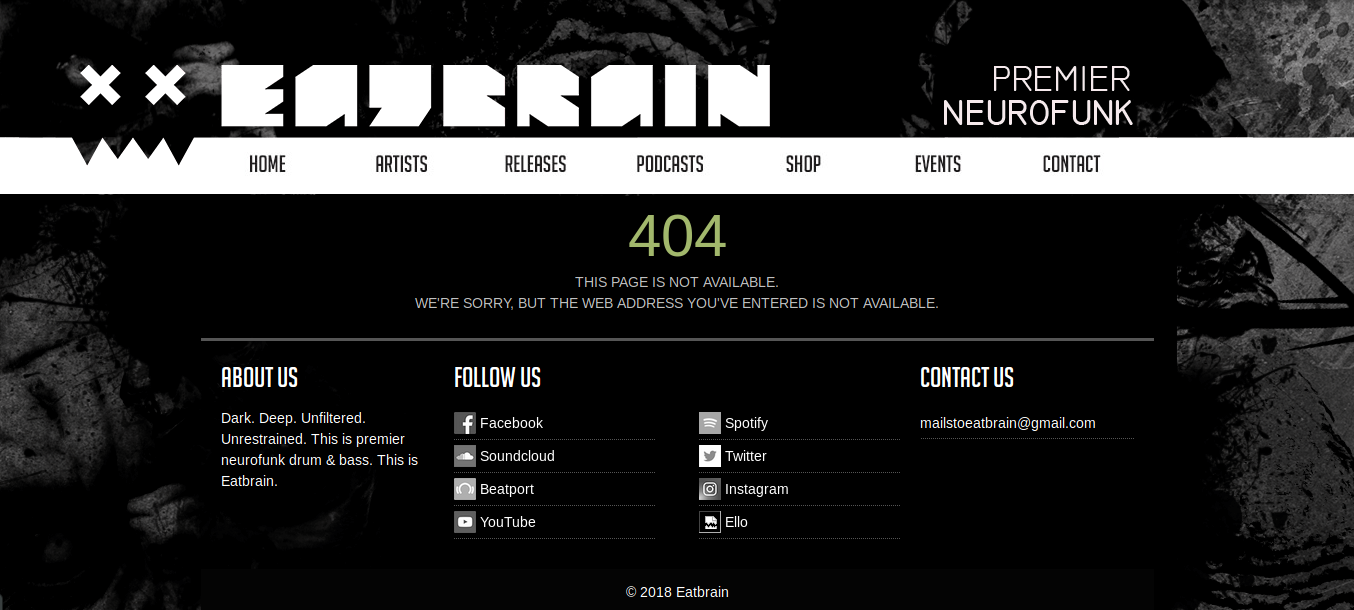
\includegraphics[width=12cm]{immagini/404}
	\caption{Pagina di Errore 404}
	\label{page-404}
\end{figure}\\
\newpage
In caso di errore 500 (Internal Server Error) invece la situazione non è gestita al meglio: la pagina infatti si presenta come testo nero su bianco (pare una leggera personalizzazione della pagina standard del Webserver Apache) e nonostante segua i dettami delle informazioni da fornire in questo caso (cosa può aver causato l'errore, contatti per sistemare la situazione, etc.), la completa discrepanza con il design usuale del sito potrebbe invogliare l'utente a non leggere il testo e a considerare il sito non funzionante.\\
\begin{figure}[h]
	\centering
	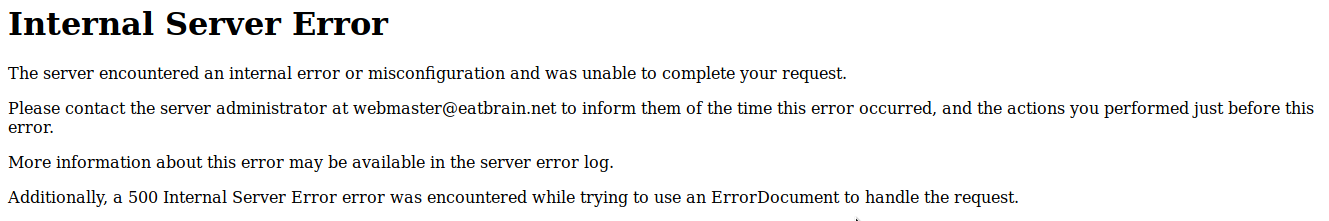
\includegraphics[width=12cm]{immagini/500}
	\caption{Pagina di Errore 500}
	\label{page-500}
\end{figure}\\
Sebbene gli errori di questo tipo siano rari, sarebbe stato meglio uniformare il messaggio d'errore con il resto del sito. \\
In più ho trovato due casi "pericolosi" in cui si presenta l'errore: gli URL del sito sono scritti nella forma: \texttt{https://eatbrain.net/resto}; ponendo invece uno slash alla fine (\texttt{https://eatbrain.net/resto/}) si incorre nell'errore sopracitato. \\
Questa piccolezza può rivelarsi più grave del previsto: se eventuali entità linkassero delle pagine del sito ponendo uno slash alla fine (che per convenzione uno potrebbe fare, di solito gli URL funzionano anche con lo slash finale), gli utenti che cliccherebbero sul link si troverebbero una pagina bianca, eliminando quasi totalmente ogni possibilità di continuare la navigazione.\\
Effettuando lo stesso errore (slash finale) ma linkando una pagina che non esiste, la situazione è ancora peggiore: viene caricata la pagina 404 ma senza alcuno stile, infondendo all'utente l'idea che il sito sia non funzionante.\\
\begin{figure}[h]
	\centering
	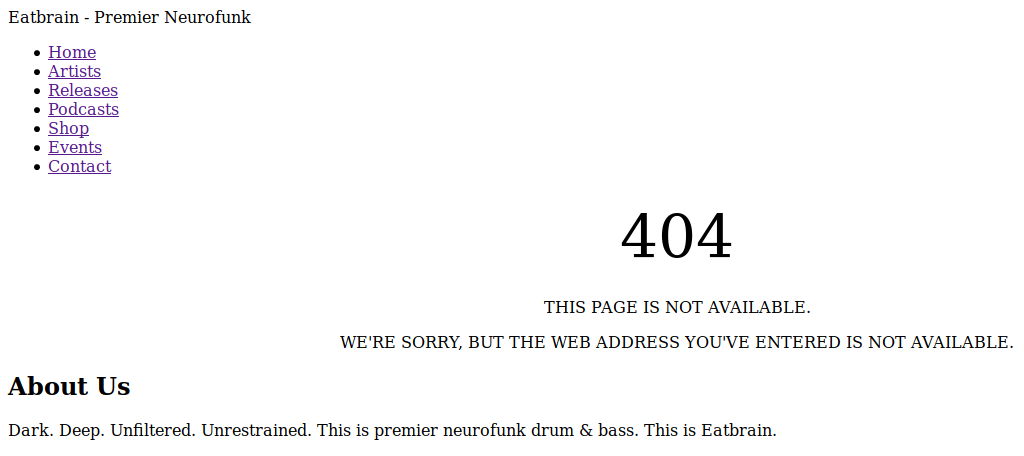
\includegraphics[width=12cm]{immagini/404-bad}
	\caption{Pagina 404 senza CSS}
	\label{page-404-bad}
\end{figure}\\ 
\subsection{Pubblicità}
Non essendo il sito web la fonte di introito per l'azienda, nessuna pagina presenta pubblicità, rendendo sicuramente più piacevole l'esperienza dell'utente.